\documentclass{article}
\usepackage[utf8]{inputenc}

\title{CSE3666 — Homework 6}
\author{Mike Medved}
\date{April 9th, 2022}

\usepackage{svg}
\usepackage{color}
\usepackage{caption}
\usepackage{amsthm}
\usepackage{amssymb} 
\usepackage{amsmath}
\usepackage{listings}
\usepackage{listings}
\usepackage{graphicx}
\usepackage[margin=1in]{geometry} 
\usepackage[scaled=0.85]{FiraMono}
\newcommand*\BitAnd{\mathbin{\&}}
\newcommand*\BitOr{\mathbin{|}}
\newcommand*\ShiftLeft{\ll}
\newcommand*\ShiftRight{\gg}
\newcommand*\BitNeg{\ensuremath{\mathord{\sim}}}

\lstdefinelanguage{Assembler}{%
  % so listings can detect directives and register names
  alsoletter={.\$},
  % strings, characters, and comments
  morestring=[b]",
  morestring=[b]',
  morecomment=[l]\#,
  % instructions
  morekeywords={[1]abs,abs.d,abs.s,add,add.d,add.s,addi,addiu,addu,%
    and,andi,auipc,b,bc1f,bc1t,beq,beqz,bge,bgeu,bgez,bgezal,bgt,bgtu,%
    bgtz,ble,bleu,blez,blt,bltu,bltz,bltzal,bne,bnez,break,c.eq.d,%
    c.eq.s,c.le.d,c.le.s,c.lt.d,c.lt.s,ceil.w.d,ceil.w.s,clo,clz,%
    cvt.d.s,cvt.d.w,cvt.s.d,cvt.s.w,cvt.w.d,cvt.w.s,div,div.d,div.s,%
    divu,ecall,eret,floor.w.d,floor.w.s,j,jal,jalr,jr,l.d,l.s,la,lb,lbu,%
    ld,ldc1,lh,lhu,li,ll,lui,lw,lwc1,lwl,lwr,madd,maddu,mfc0,mfc1,%
    mfc1.d,mfhi,mflo,mov.d,mov.s,move,movf,movf.d,movf.s,movn,movn.d,%
    movn.s,movt,movt.d,movt.s,movz,movz.d,movz.s,msub,msubu,mtc0,mtc1,%
    mtc1.d,mthi,mtlo,mul,mul.d,mul.s,mulo,mulou,mult,multu,mulu,mv,neg,%
    neg.d,neg.s,negu,nop,nor,not,or,ori,rem,remu,rol,ror,round.w.d,%
    round.w.s,s.d,s.s,sb,sc,sd,sdc1,seq,sge,sgeu,sgt,sgtu,sh,sle,%
    sleu,sll,slli,sllv,slt,slti,sltiu,sltu,sne,sqrt.d,sqrt.s,sra,srai,srav,srl,%
    srlv,sub,sub.d,sub.s,subi,subiu,subu,sw,swc1,swl,swr,syscall,teq,%
    teqi,tge,tgei,tgeiu,tgeu,tlt,tlti,tltiu,tltu,tne,tnei,trunc.w.d,%
    trunc.w.s,ulh,ulhu,ulw,ush,usw,xor,xori},
  % assembler directives
  morekeywords={[2].align,.ascii,.asciiz,.byte,.data,.double,.extern,%
    .float,.globl,.half,.kdata,.ktext,.set,.space,.text,.word},
  % register names
  morekeywords={[3]\$0,\$1,\$2,\$3,\$4,\$5,\$6,\$7,\$8,\$9,\$10,\$11,%
    \$12,\$13,\$14,\$15,\$16,\$17,\$18,\$19,\$20,\$21,\$22,\$23,\$24,%
    \$25,\$26,\$27,\$28,\$29,\$30,\$31,%
    \$zero,\$at,\$v0,\$v1,\$a0,\$a1,\$a2,\$a3,\$t0,\$t1,\$t2,\$t3,\$t4,
    \$t5,\$t6,\$t7,\$s0,\$s1,\$s2,\$s3,\$s4,\$s5,\$s6,\$s7,\$t8,\$t9,%
    \$k0,\$k1,\$gp,\$sp,\$fp,\$ra},
}[strings,comments,keywords]

\definecolor{CommentGreen}{rgb}{0,.6,0}
% \lstset{
%   language=[mips]Assembler,
%   escapechar=@, % include LaTeX code between `@' characters
%   keepspaces,   % needed to preserve spacing with lstinline
%   basicstyle=\small\ttfamily\bfseries,
%   commentstyle=\color{CommentGreen},
%   stringstyle=\color{cyan},
%   showstringspaces=false,
%   keywordstyle=[1]\color{blue},    % instructions
%   keywordstyle=[2]\color{magenta}, % directives
%   keywordstyle=[3]\color{red},     % registers
% }

\lstset{basicstyle=\ttfamily, keywordstyle=\bfseries}
\lstset{
    % language=Python,
    aboveskip=3mm,
    belowskip=3mm,
    showstringspaces=false,
    columns=flexible,
    basicstyle={\small\ttfamily},
    numbers=none,
    numberstyle=\tiny\color{gray},
    keywordstyle=\color{blue},
    commentstyle=\color{dkgreen},
    stringstyle=\color{mauve},
    breaklines=true,
    breakatwhitespace=true,
    tabsize=3
}

\definecolor{dkgreen}{rgb}{0,.6,0}
\definecolor{mauve}{rgb}{224,176,255}

\begin{document}

\maketitle

\section{Question 2a}
We first change part of diagram shown in the following figure. The goal is to set the correct next PC value at the output of Mux3. We will need a new Mux. We call it Mux4. The output of Mux4 is PCRef (the reference PC). In addition, we need to change how the select signal of Mux3 is generated. Let us call the new select signal PCSrcJ. Include the following in your submission. Your diagram must be clean.

\section{Deliverable}
    \scalebox{1.0}{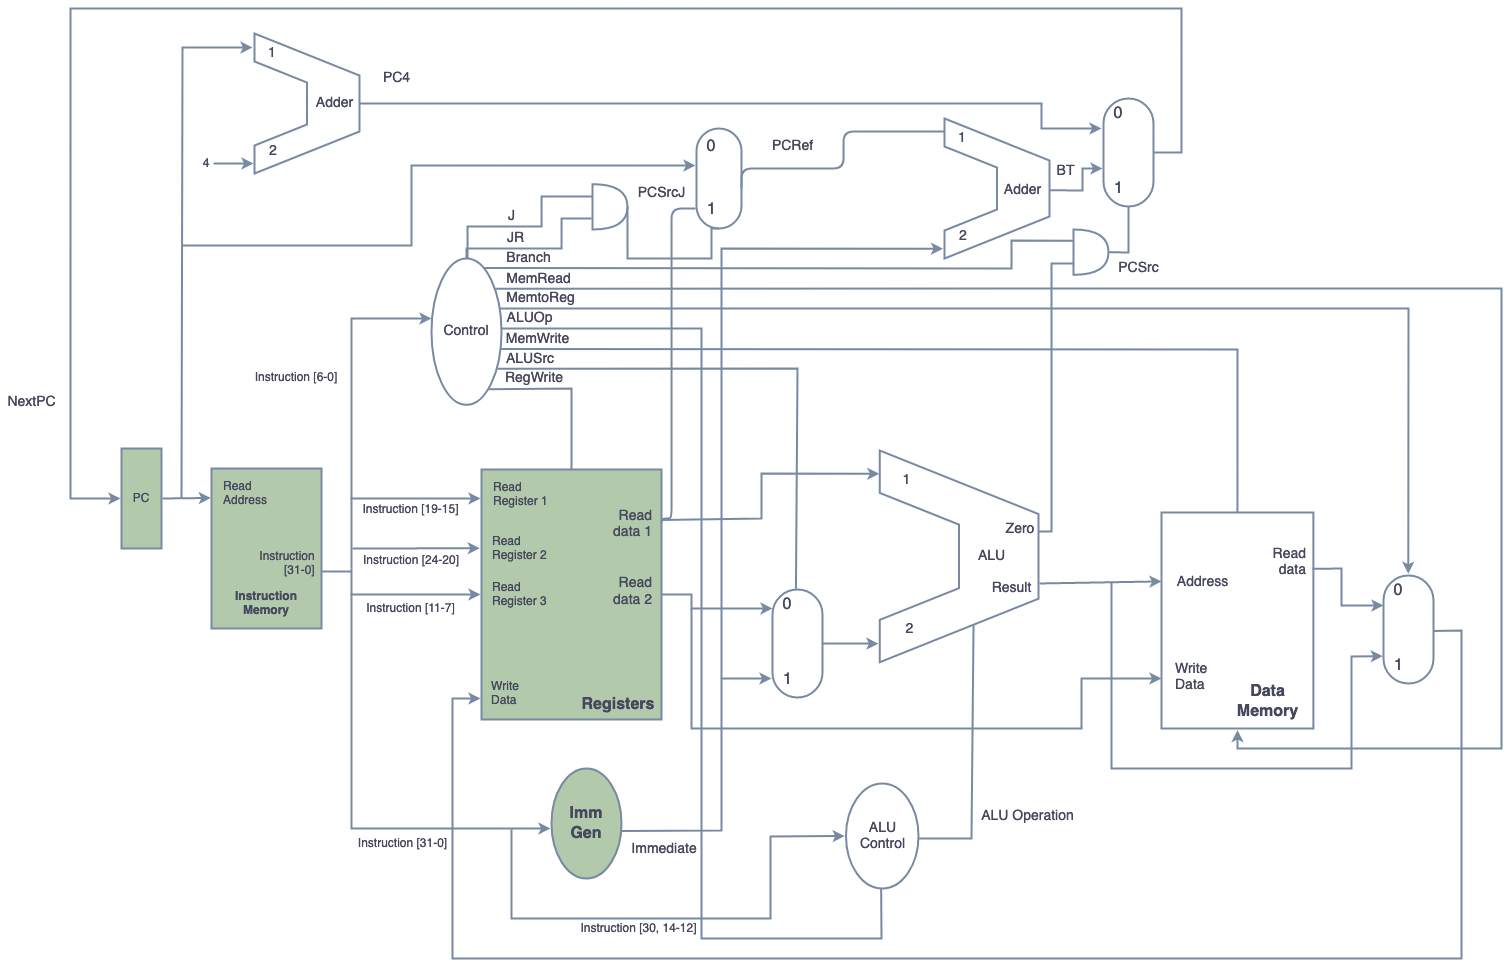
\includegraphics[width=\textwidth]{./3666-q2a.png}}

\break
\section{Question 2b}
We then change part of diagram shown in the following figure. The goal is to set the correct value on Write Data. We will need to add a Mux. Let us call it Mux 5. The output of Mux5, ExResult, is connected to input 0 of Mux2. Mux5 is controlled by an existing signal (i.e., there is no need to add logic to generate the select signal of Mux5). Draw a new diagram that includes Mux5. Label every signal in your diagram. Your diagram must be clean.

\section{Deliverable}
    \scalebox{1.0}{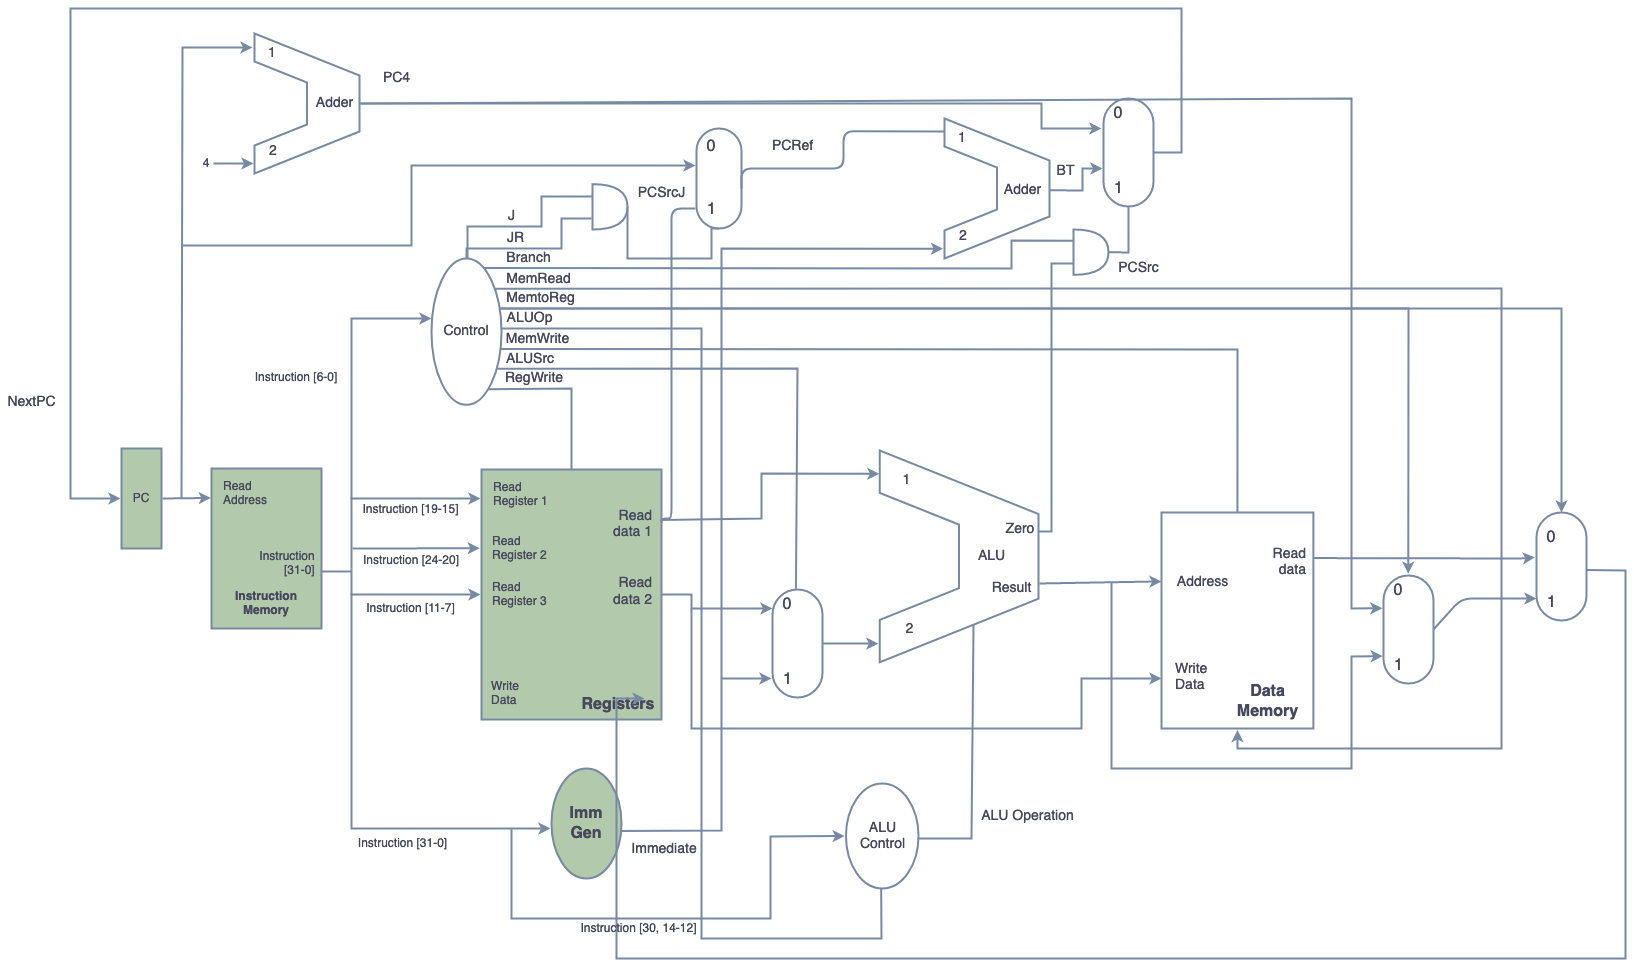
\includegraphics[width=\textwidth]{./3666-q2b.png}}


\end{document}
